\section{Radice reale di curve depresse}
\label{compl:cubidepresse}
Si consideri la seguente equazione cubica tipo\footnote{Equazioni cubiche di questo tipo sono dette \emph{depresse}, in quanto mancano del termine di secondo grado.}:
\begin{equation}
	\label{compl:iniziale}
	x^3+px=q
\end{equation}
Per il teorema dei valori intermedi, o comunque osservando il grafico (figura \ref{compl:cubica}), si può notare che per qualunque valore dei coefficienti $p$ e $q$ l'equazione ammette almeno una soluzione reale. È naturale dunque chiedersi se esista una formula risolutiva che trovi la radice reale per tutte le equazioni di questo tipo.

\begin{figure}[ht]
	\centering
	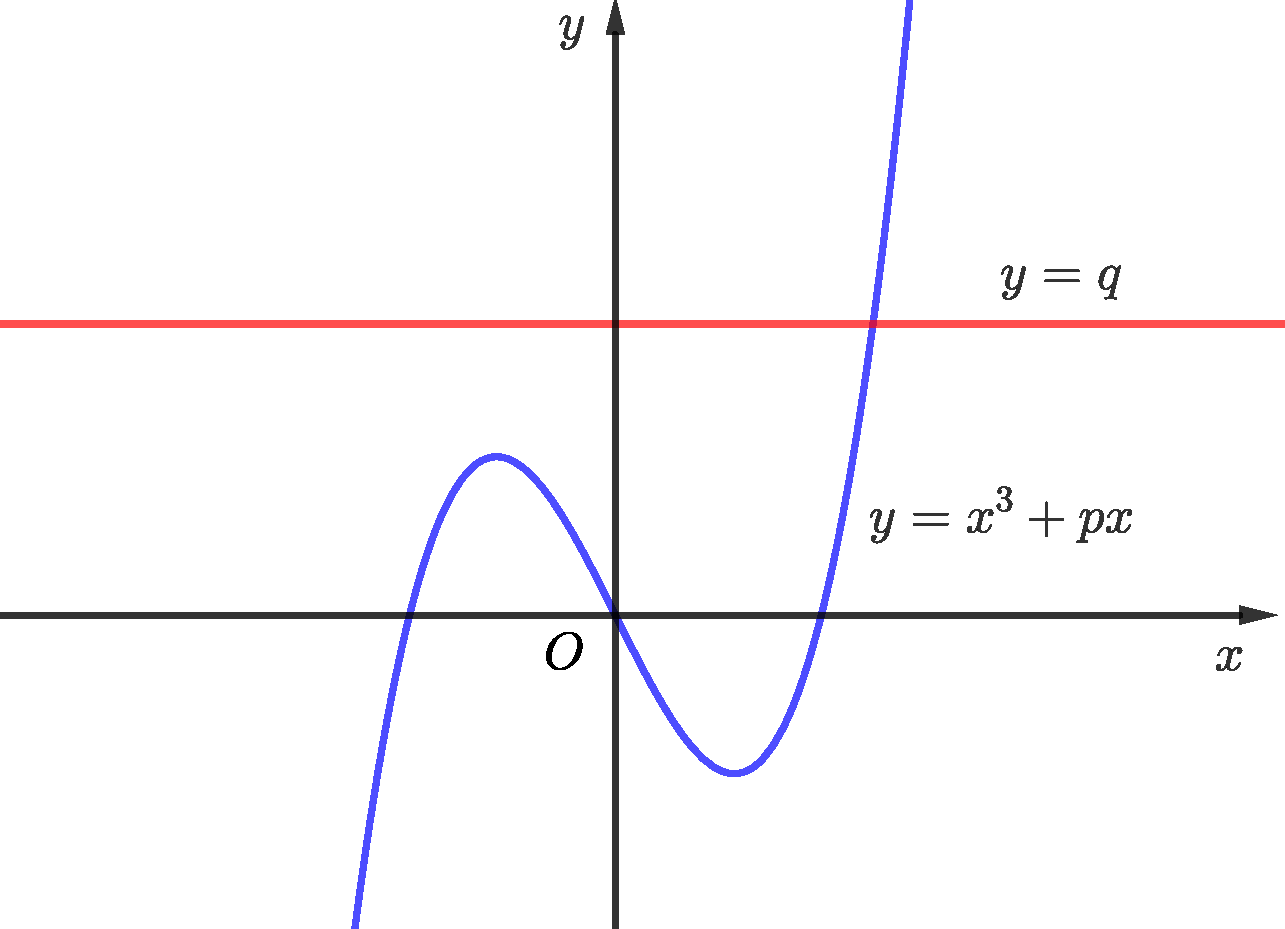
\includegraphics[width=0.8\textwidth]{grafici/cubica}
	\caption{L'equazione \ref{compl:iniziale} rappresentata graficamente tramite le funzioni $y=x^3+px$ e $y=q$.}
	\label{compl:cubica}
\end{figure}

\begin{proof}
	Partendo dalla \ref{compl:iniziale}, pongo $x=u+v$.
	\begin{align}
		(u+v)^3+p (u+v)            & = q \notag                  \\
		u^3+3u^2v+3uv^2+v^3+p(u+v) & = q \notag                  \\
		u^3+v^3+(3uv+p)(u+v)       & = q \label{compl:raddoppia}
	\end{align}
	La sostituzione $x = u + v$ non impone alcuna unicità, fissato il valore di $x$, delle due incognite sostitutive (l'equazione sostitutiva ha infinite soluzioni). Questo permette di scegliere una seconda relazione, per esempio che annulli il fattore $3uv + p$, che va a formare con la prima un sistema lineare in due equazioni in due incognite che, fissato $x$, ammette una e una sola soluzione (valori unici per $u$ e $v$):
	\begin{equation}
		\label{compl:sostsist}
		\begin{cases}
			x = u + v \\
			3uv + p = 0
		\end{cases}
	\end{equation}
	La relazione scelta permette di semplificare notevolmente l'equazione \ref{compl:raddoppia}, che si può ora esprimere tramite il sistema:
	\begin{subequations}
		\begin{numcases}{}
			3uv+p=0 \notag \\
			u^3+v^3=q \label{compl:u3v3}
		\end{numcases}
		\begin{numcases}{}
			v=-p/3u \notag \\
			u^3-\dfrac{p^3}{27u^3}=q \label{compl:quadratica-nascosta}
		\end{numcases}
	\end{subequations}
	Prendendo in considerazione l'equazione \ref{compl:quadratica-nascosta} e moltiplicando entrambi i membri\footnote{Risolvendo in $u$ il sistema \ref{compl:sostsist} si può notare che la variabile non è mai nulla, poiché supposto $p \neq 0$.} per $u^3$:
	\begin{align}
		u^3-\frac{p^3}{27u^3}-q     & = 0 \notag \\
		(u^3)^2-qu^3-\frac{p^3}{27} & = 0 \notag
	\end{align}
	Interpreto come un'equazione quadratica in $u^3$ e risolvo:
	\begin{gather}
		u^3=\frac{q\pm\sqrt{q^2+\dfrac{4p^3}{27}}}{2}= \notag \\ =\frac{q}{2}\pm\frac{1}{2}\sqrt{q^2+\frac{4p^3}{27}}= \notag \\
		=\frac{q}{2}\pm\sqrt{\frac{1}{4}\left(q^2+\frac{4p^3}{27}\right)}= \notag \\ =\frac{q}{2}\pm\sqrt{\left(\frac{q}{2}\right)^2+\left(\frac{p}{3}\right)^3}
	\end{gather}
	dove il radicando $\left(\frac{q}{2}\right)^2+\left(\frac{p}{3}\right)^3$ è detto discriminante ($\Delta$) dell'equazione iniziale (\ref{compl:iniziale}). Per $v^3$ si ottiene un risultato simmetrico, come si può dimostrare sfruttando l'uguaglianza \ref{compl:u3v3}:
	\[
		v^3 = q - u^3 = q - \left(\frac{q}{2} \pm \sqrt{\left(\frac{q}{2}\right)^2 + \left(\frac{p}{3}\right)^3}\right) = \frac{q}{2} \mp \sqrt{\left(\frac{q}{2}\right)^2 + \left(\frac{p}{3}\right)^3}
	\]
	In altre parole, quando si applica il più per $u$ si applica il meno per $v$ e viceversa. Tornando alla variabile $x=u+v$ risolvo l'equazione iniziale (scelgo un segno qualunque, pur mantenendo la coerenza tra i due, in quanto la somma è commutativa):
	\begin{equation}
		x = u + v = \sqrt[3]{\frac{q}{2} + \sqrt{\left(\frac{q}{2}\right)^2+\left(\frac{p}{3}\right)^3}}+\sqrt[3]{\frac{q}{2}-\sqrt{\left(\frac{q}{2}\right)^2+\left(\frac{p}{3}\right)^3}} \label{compl:risolutiva}
	\end{equation}
\end{proof}
\begin{examp}
	\begin{gather*}
		x^3 + 6x = 20 \\
		\Delta = \left( \frac{q}{2} \right)^2 + \left( \frac{p}{3} \right)^3 = \left( \frac{20}{2} \right)^2 + \left( \frac{6}{3} \right)^3 = 10^2 + 2^3 = 108 \\
		x = \sqrt[3]{10 + \sqrt{108}} + \sqrt[3]{10 - \sqrt{108}}
	\end{gather*}
	Ma
	\begin{align*}
		(1 \pm \sqrt3)^3 & =                                                                     \\
		                 & = 1^3 \pm 3 \cdot 1^2 \cdot \sqrt3 + 3 \cdot 1 \cdot (\pm \sqrt 3 )^2 \\
		                 & = 1 \pm 3 \sqrt 3 + 9 \pm 3 \sqrt 3                                   \\
		                 & = 10 \pm \sqrt{108}
	\end{align*}
	Quindi
	\[
		x=\sqrt[3]{10+\sqrt{108}}+\sqrt[3]{10-\sqrt{108}}=1+\sqrt3+1-\sqrt3=2
	\]
\end{examp}
La peculiarità della formula \ref{compl:risolutiva} è che permette di trovare la radice reale anche quando il discriminante è negativo. Infatti, applicando un ragionamento analogo a quello dell'esempio:
\begin{gather*}
	x^3 - 15x = 4 \\
	\Delta=\left(\frac{q}{2}\right)^2+\left(\frac{p}{3}\right)^3=\left(\frac{4}{2}\right)^2+\left(\frac{-15}{3}\right)^3=2^2+(-5)^3=-121 < 0 \\
	x=\sqrt[3]{2+\sqrt{-121}}+\sqrt[3]{2-\sqrt{-121}}
\end{gather*}
Il simbolo $\sqrt{-121}$ non ha significato. Tuttavia si può pensare di estendere la proprietà per cui $(\sqrt{a})^2=a$:
\begin{gather*}
	( 2 \pm \sqrt{-1} )^3 = 8 + 3*4( \pm \sqrt{-1} ) + 3*2( \pm \sqrt{-1} )^2 + ( \pm \sqrt{-1} )^3 = \\
	8 \pm 12\sqrt{-1} + 6(-1) + (-1)( \pm \sqrt{-1} ) = 2 \pm 11\sqrt{-1} = 2 \pm \sqrt{-121}
\end{gather*}
Quindi
\[
	x=\sqrt[3]{2+\sqrt{-121}}+\sqrt[3]{2-\sqrt{-121}}=2+\sqrt{-1}+2-\sqrt{-1}=4
\]
In questo modo senza comprendere il significato del simbolo $\sqrt{-1}$ possiamo ricavare la radice reale.
